\documentclass[11pt]{article}

% Change "review" to "final" to generate the final (sometimes called camera-ready) version.
% Change to "preprint" to generate a non-anonymous version with page numbers.
\usepackage[preprint]{acl}

% Standard package includes
\usepackage{times}
\usepackage{latexsym}
\usepackage[T1]{fontenc}
\usepackage[utf8]{inputenc}
\usepackage{microtype}
\usepackage{inconsolata}
\usepackage{graphicx}
\usepackage{booktabs}
\usepackage{amsfonts}
\usepackage{nicefrac}
\usepackage{enumitem}
\usepackage{multirow}

\title{Can Budget Models Write Sakha? A Cross-Lingual Evaluation of Under-Resourced Text Generation}

% In review mode, use anonymous author
\author{Nikolai Neustroev \\
  \texttt{n.neustroev@web.de} \\}

\begin{document}
\maketitle


\begin{abstract}
Sakha (Yakut) is an under-resourced Turkic language with a limited digital presence.
We evaluate four cost-efficient models (DeepSeek V3.2, Qwen 3.5-Flash, Gemini 3.1 Flash-Lite, and GPT-5.4 Nano) on a sentence-continuation task derived from the Universal Declaration of Human Rights, using zero-, one-, and few-shot prompting across six languages spanning the full resource spectrum.
Gemini 3.1 Flash-Lite leads on all metrics and is the most consistent.
GPT-5.4 Nano scores lowest with high variance.
Sakha ranks 5th of 6 languages, well above Central Kanuri but significantly below Icelandic and Kazakh.
A pronounced Char F1 / Word F1 gap, unique to Sakha and Kanuri, suggests models are generating rather than recalling the reference text, reflecting limited training exposure.
One-shot prompting yields a significant improvement over zero-shot, but the direction and magnitude of the effect is model-dependent.
\end{abstract}


\section{Introduction}
Sakha (Yakut) is the language of an Indigenous Turkic people of northeastern Asia, spoken by approximately 378,000 people, with a sparse digital footprint.
As large language models are increasingly deployed in multilingual settings, understanding their capabilities on such languages is both practically and scientifically important: practically because speakers of under-resourced languages stand to benefit from or be failed by these systems, and scientifically because under-resourced languages provide a controlled setting for isolating the effect of training data availability from architectural and capability differences.
This paper evaluates four recently released, cost-efficient LLMs on Sakha text generation, benchmarks their performance against five control languages across the resource spectrum, and examines the effect of few-shot prompting on model behavior.

\subsection{Literature review}
This review evaluates existing approaches and findings on LLM performance for under-resourced languages, with particular attention to the factors that drive capability gaps.
The global linguistic landscape consists of over 7,000 languages, yet over 90\% of these are under-studied by the NLP community \cite{joshi-etal-2020-state}, and approximately 43\% are threatened with extinction through marginalization by globalization, urbanization, and dominant languages \cite{vasconcelos2024disappearing, zhong2026opportunitieschallengeslargelanguage}.
This neglect is structural: the majority of modern evaluation frameworks and digital resources are predominantly English-centric, driven by the availability of high-quality digital text \cite{lai-etal-2024-llms}.

Within this landscape, two performance factors emerge consistently across prior work.
First, training data availability is a primary driver of model capability: a model's performance on under-resourced languages correlates directly with the amount of monolingual data available on the web, so languages with more web presence (e.g.\ Swahili) achieve significantly better results than severely under-resourced languages (e.g.\ Wolof) \cite{ojo-etal-2025-afrobench}.
Second, morphological complexity compounds the challenge: as word-form complexity increases, LLM performance drops sharply while human performance remains robust \cite{ismayilzada-etal-2025-evaluating}, a finding directly relevant to agglutinative languages such as Sakha.
Even proprietary models, which consistently outperform open-source alternatives on under-resourced benchmarks \cite{ojo-etal-2025-afrobench, jayakody2024performancerecentlargelanguage}, struggle with culturally grounded reasoning and region-specific knowledge for non-English languages \cite{toraman-etal-2026-turkbench}.

Few-shot prompting offers a practical lever for mitigating these gaps.
Providing demonstration examples has been shown to dramatically improve performance on African languages across tasks such as Automatic Diacritics Restoration and math reasoning \cite{ojo-etal-2025-afrobench}, and evaluations on Bengali similarly find that few-shot prompting generally yields the best results by helping models adapt through contextual examples \cite{nazi_evaluation_2025}.
This evidence supports our choice to evaluate zero-, one-, and few-shot conditions and to treat prompting strategy as an independent variable alongside model selection.

\section{Methods}

\subsection{Model selection}
The four models selected for this study (DeepSeek V3.2 \cite{deepseekai2025deepseekv32}, Qwen 3.5-Flash \cite{qwen3.5}, Gemini 3.1 Flash-Lite Preview \cite{gemini3.1}, and GPT-5.4 Nano \cite{gpt5.4}) fall within the sub-\$0.30 per-million-input-token pricing band, ensuring a fair cost-aware comparison.
Each is from an independent organisation, reducing the risk of provider bias.
The pool reflects architectural variation, ranging from large-scale sparse Mixture-of-Experts (MoE) to hybrid linear-attention MoE, knowledge-distilled, and natively compact dense designs.
It also balances open-weight models (DeepSeek under MIT, Qwen under Apache 2.0) against closed-weight API-only models.
DeepSeek V3.2, despite sharing the pricing tier, operates at frontier-class capability and therefore serves as an internal anchor model against which the three lightweight models can be calibrated.
These choices are a trade-off: by constraining the pool to the sub-\$0.30 pricing tier, the design does not cover dedicated frontier and mid-tier models, limiting coverage of the full cost-quality curve.
We also accept a reproducibility risk in the inclusion of Gemini 3.1 Flash-Lite, whose preview status means its behaviour may change before general availability.

\begin{table*}[ht]
    \centering
    \caption{Models}
    \label{tab:model_comparison}
    \small
    \begin{tabular*}{\textwidth}{@{\extracolsep{\fill}}lllllll@{}}
        \toprule
        \textbf{Model} & \textbf{Release} & \textbf{Context} & \textbf{In*} & \textbf{Out*} & \textbf{Architecture} & \textbf{License} \\
        \midrule
        DeepSeek V3.2 & Dec 2025 & 164K & \$0.28 & \$0.42 & Sparse MoE & MIT \\
        Qwen 3.5-Flash & Feb 2026 & 1M & \$0.10 & \$0.40 & Hybrid Linear MoE & Apache 2.0 \\
        Gemini 3.1 & Mar 2026 & 1M+ & \$0.25 & \$1.50 & Distilled & Prop. \\
        GPT-5.4 Nano & Mar 2026 & 400K & \$0.20 & \$1.25 & Compact Dense & Prop. \\
        \bottomrule
    \end{tabular*}
    \vspace{2pt}\\
    \small *Prices in USD per 1 million tokens.
\end{table*}

\subsection{Control selection}
Sakha is an under-resourced language and to understand how the models perform on it we need to compare their performance on different languages.
Researchers classify languages onto six classes based on resource availability, where Class 0 are languages "with exceptionally limited resources" and Class 5 are "quintessential rich-resource languages"\cite{joshi-etal-2020-state}.
Sakha belongs to Class 1.
We use English as our Class 5, Korean as Class 4, Kazakh as Class 3, Icelandic as Class 2 and Central Kanuri as Class 0 control languages.

\begin{table*}[ht]
    \centering
    \caption{Language resource profiles}
    \label{tab:language_resources}
    \small
    \begin{tabular*}{\textwidth}{@{\extracolsep{\fill}}clrrrrr@{}}
        \toprule
        \textbf{Class} & \textbf{Language} & \textbf{Speakers}& \textbf{DLS Score} & \textbf{Wikipedia} & \textbf{GlotCC} & \textbf{CommonCrawl} \\
        \midrule
        0 & Central Kanuri & $\sim$ 9\,298\,000 & 0.46 & 1\,634 & 14 & Undoc. \\
        1 & Sakha & $\sim$ 378\,000 & 0.50 & 18\,087 & 2\,445 & Undoc. \\
        2 & Icelandic & $\sim$ 325\,620 & 0.86 & 60\,924 & 409\,042 & 0.0383\% \\
        3 & Kazakh & $\sim$ 16\,589\,620 & 0.82 & 242\,884 & 200\,185 & 0.0380\% \\
        4 & Korean & $\sim$ 81\,652\,230 & 0.96 & 741\,653 & $\sim$ 2\,830\,000 & 0.8378\% \\
        5 & English & $\sim$ 371\,590\,770 & 1.00 & 65\,364\,252 & $\sim$ 266\,000\,000 & 41.0588\% \\
        \bottomrule
    \end{tabular*}
    \vspace{2pt}\\
    \small Speakers = number of L1 speakers \cite{ethnologue2026}; DLS Score = Digital Language Support Score \cite{ethnologue2026, simons-etal-2022-assessing}; Wikipedia = number of articles \cite{MetaListWikipedias2026}; GlotCC = number of documents \cite{kargaran2024glotcc}; CommonCrawl = number of documents \cite{CommonCrawlStats2026}. Undoc.\ = undocumented.
\end{table*}

\subsection{Data retrieval}
The evaluation task was defined as sentence-level continuation of Article 1 of the Universal Declaration of Human Rights (UDHR)\footnote{The translation were taken from the UN High Commissioner's for Human Rights website (\url{https://www.ohchr.org/}), with exception of Kazakh version (\url{https://adilet.zan.kz/kaz/docs/O4800000001})}.
For each language, the article's opening sentence was used as the prompt seed and its remainder as the reference completion.
Additional articles (2, 4, and 7) were reserved as in-context examples for few-shot prompting.
We choose the UDHR because its parallel alignment across different languages allows controlled, cross-lingual comparisons over a consistent, uniform register, reducing noise from domain or style variation.
However, its narrow legal-political domain and small size mean evaluation scores reflect only a small part of real-world language use and carry considerable uncertainty.

Three prompting strategies were used in a fully crossed design. All prompts were in English regardless of the target language.

\begin{enumerate}
\item Zero-shot. The model received a system prompt instructing it to wrap its answer in \texttt{<answer>} tags, followed by a user message with the first sentence of Article 1 and requesting its continuation in the target language.
\item One-shot. A single completed example (Article 2) was included to the user message to demonstrate the expected input-output format before presenting the Article 1 prompt.
\item Few-shot. Three completed examples (Articles 2, 4, and 7) were included to the user message.
\end{enumerate}

All models were queried with identical hyperparameters: temperature 0.7, top\_p 1.0, maximum output length 512 tokens, and both frequency and presence penalties set to 0.0. Reasoning effort was explicitly set to \texttt{none} where supported. We accessed all models through the OpenRouter API gateway\footnote{\url{https://openrouter.ai/}}.

\subsection{Metrics}
For evaluation of models' performance we used such character-level metrics as normalized longest common subsequence (NLCS), Jaccard similarity, F1 score and word-level F1 score. We chose this set of character- and word-level string similarity metrics because they are fully tokenizer-agnostic and deterministic, ensuring fair comparison across models. However, the set is semantically blind, penalizing valid paraphrases and morphological variants equally with actual errors, and applies uniform weight to every character regardless of its semantic importance.

\section{Results}

\subsection{Which LLM performs best / worst on Sakha?}

Table~\ref{tab:model_perf} reports mean scores and 95\% confidence intervals for all models.
Gemini 3.1 Flash Lite Preview leads on every metric and is also the most consistent performer (Char F1 std\,=\,0.039, the lowest of all models; minimum Char F1 of 0.595).
GPT-5.4 Nano scores the lowest on all metrics.
Wide confidence intervals reflect high variance (std\,=\,0.184).
Some samples are handled adequately while others fail almost entirely (minimum Char F1 of 0.060).

\begin{table*}[ht]
    \centering
    \caption{Model performance on Sakha (mean [95\% CI]).}
    \label{tab:model_perf}
    \small
    \begin{tabular}{lcccc}
        \toprule
        \textbf{Model} & \textbf{Char F1} & \textbf{Word F1} & \textbf{Jaccard} & \textbf{Norm.\ LCS} \\
        \midrule
        Gemini 3.1 Flash Lite & 0.799 [0.794--0.803] & 0.270 [0.261--0.279] & 0.880 [0.875--0.886] & 0.609 [0.601--0.618] \\
        DeepSeek V3.2         & 0.781 [0.775--0.786] & 0.102 [0.095--0.109] & 0.815 [0.807--0.823] & 0.462 [0.454--0.470] \\
        Qwen 3.5 Flash        & 0.704 [0.687--0.720] & 0.083 [0.078--0.088] & 0.740 [0.730--0.750] & 0.368 [0.357--0.379] \\
        GPT-5.4 Nano          & 0.650 [0.630--0.671] & 0.065 [0.059--0.071] & 0.659 [0.639--0.680] & 0.304 [0.293--0.315] \\
        \bottomrule
    \end{tabular}
\end{table*}

\begin{figure*}[h]
    \centering
    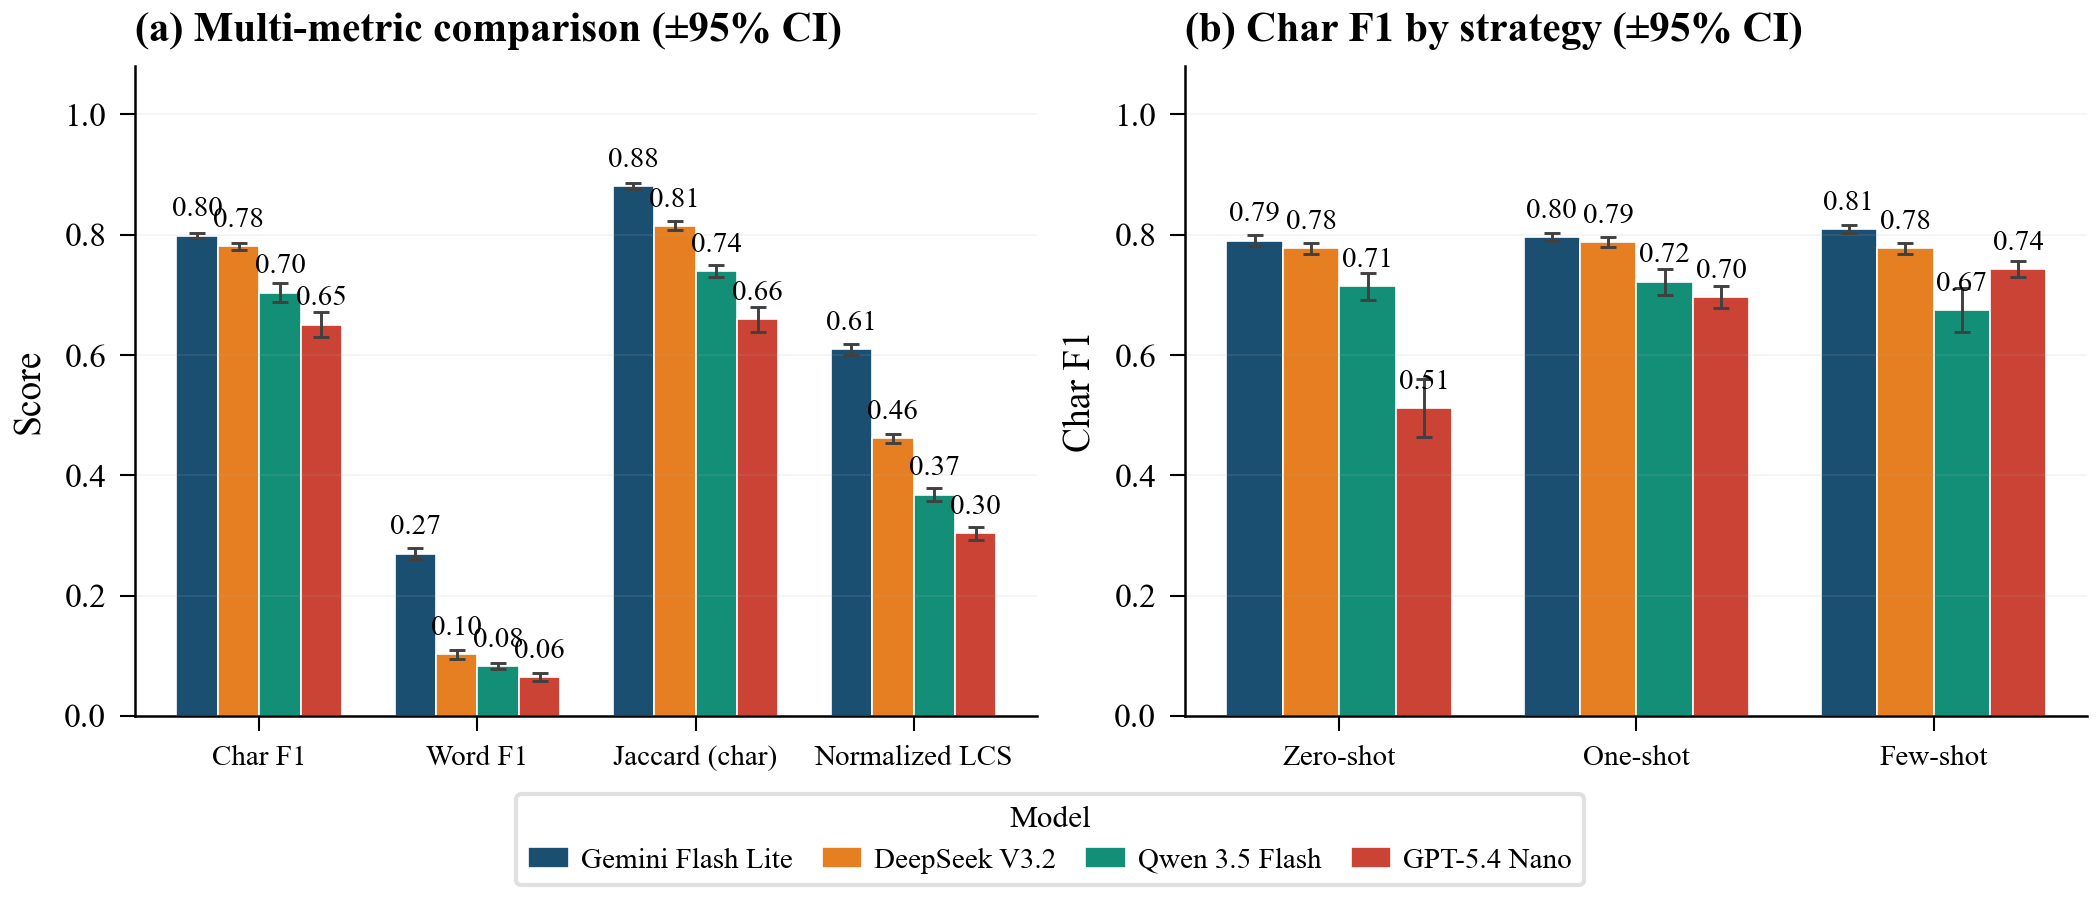
\includegraphics[width=1.0\textwidth]{plot1_sakha_model_comparison.png}
    \caption{LLM performance on Sakha}
    \label{fig:plot1_sakha_model_comparison}
\end{figure*}

All pairwise Char F1 rankings are statistically significant at 95\% confidence (Table~\ref{tab:pairwise}).
The low Gemini--DeepSeek gap is significant too, driven by both models' low variance.
DeepSeek vs.\ Qwen and DeepSeek vs.\ GPT are also significantly different by similar margins.

\begin{table}[ht]
    \centering
    \caption{Pairwise Char F1 gaps on Sakha (all significant at $p < 0.05$).}
    \label{tab:pairwise}
    \small
    \begin{tabular}{lcc}
        \toprule
        \textbf{Pair} & \textbf{Gap} & \textbf{95\% CI} \\
        \midrule
        Gemini vs.\ DeepSeek & +0.018 & [+0.011,\ +0.025] \\
        Gemini vs.\ Qwen     & +0.095 & [+0.078,\ +0.112] \\
        Gemini vs.\ GPT      & +0.148 & [+0.123,\ +0.174] \\
        \bottomrule
    \end{tabular}
\end{table}

DeepSeek V3.2 ranks second and is close to Gemini on character-level metrics, but drops sharply on Word F1, suggesting it captures surface character patterns without reliably reconstructing whole words.
Qwen 3.5 Flash ranks third, with wider confidence intervals.

All four models show a large gap between character-level scores (Char F1, Jaccard) and word-level scores (Word F1) on Sakha. The best Word F1 is only 27\% (Gemini), compared to 95\%+ on English.
This means the best model's output diverges from the reference at the word level, despite reasonable character-level overlap.
Word F1 measures exact matches, so in an agglutinative language like Sakha it may conflate genuine errors (wrong vocabulary, mistranslations) with valid alternative morphological forms.
The UDHR setting limits this concern somewhat: there is one canonical reference translation, so consistent word-level divergence does signal real difficulty in faithfully reproducing it.
But the gap between Char F1 and Word F1 should be read as \textit{``the model struggles to match the exact reference wording''} rather than \textit{``a non-matching word is an error.''}

\subsection{Does one-shot and few-shot improve performance on Sakha?}

On average, one-shot provides a statistically significant boost over zero-shot. The additional step from one-shot to few-shot is negligible and not significant overall.
The effect is highly model-dependent (see table~\ref{tab:strategy} for Char F1 per model and strategy).

\begin{table*}[ht]
    \centering
    \caption{Char F1 by model and prompting strategy on Sakha (mean [95\% CI]).}
    \label{tab:strategy}
    \small
    \begin{tabular}{lccc}
        \toprule
        \textbf{Model} & \textbf{Zero-shot} & \textbf{One-shot} & \textbf{Few-shot} \\
        \midrule
        Gemini 3.1 Flash Lite & 0.790 [0.781--0.800] & 0.796 [0.790--0.803] & 0.809 [0.803--0.816] \\
        DeepSeek V3.2         & 0.777 [0.768--0.787] & 0.787 [0.779--0.796] & 0.777 [0.768--0.787] \\
        Qwen 3.5 Flash        & 0.714 [0.691--0.737] & 0.722 [0.701--0.743] & 0.675 [0.638--0.712] \\
        GPT-5.4 Nano          & 0.512 [0.464--0.560] & 0.696 [0.678--0.714] & 0.743 [0.729--0.756] \\
        \bottomrule
    \end{tabular}
\end{table*}

\begin{figure}[h]
    \centering
    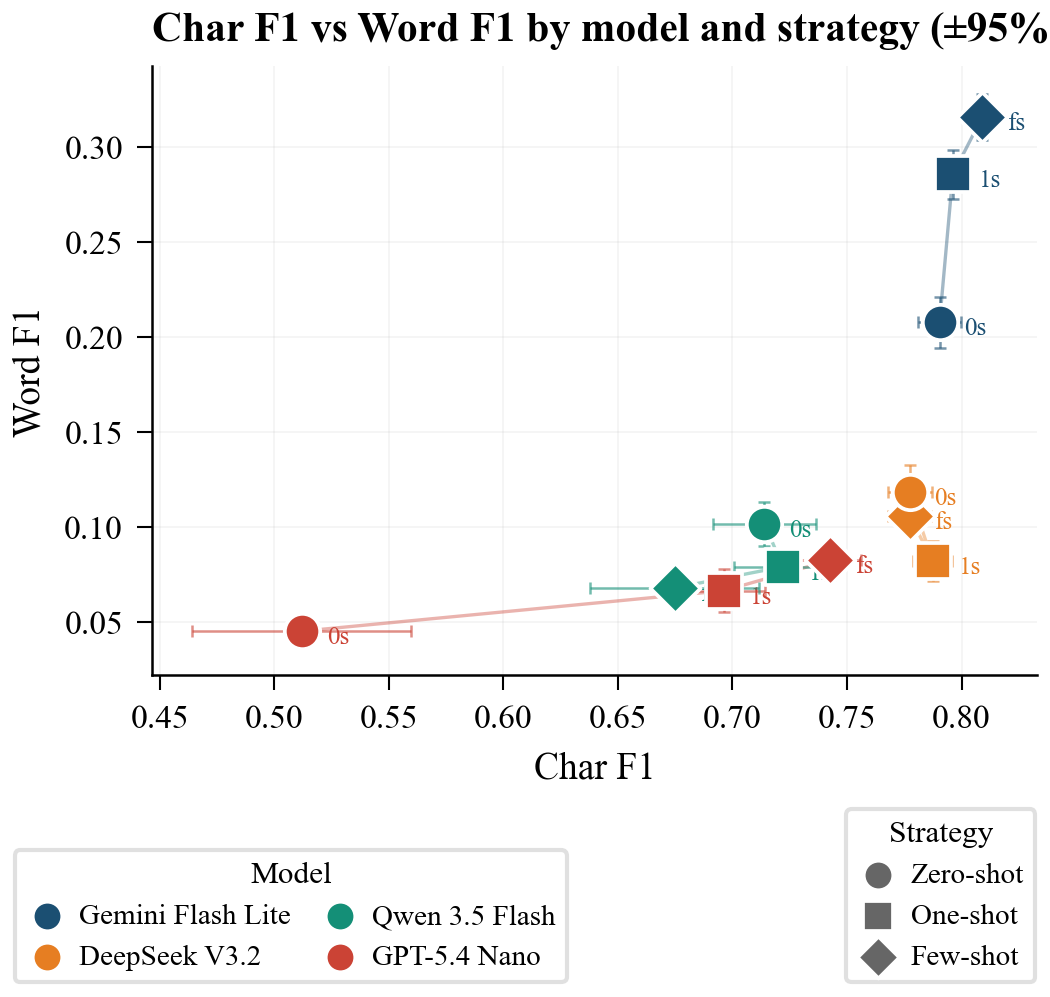
\includegraphics[width=\columnwidth]{plot2_sakha_strategy_scatter.png}
    \caption{Strategy influence on performance in Sakha}
    \label{fig:plot2_sakha_strategy_scatter}
\end{figure}

GPT-5.4 Nano benefits the most from examples which yield a meaningful, statistically credible gain.
Gemini shows modest but significant improvement with small gains because it already performs well in zero-shot, and the Word F1 trend is consistent ($0.208 \to 0.286 \to 0.316$).
DeepSeek V3.2 is essentially flat across strategies, examples neither help nor hurt.
Qwen 3.5 Flash shows a directionally negative trend with few-shot: the confidence interval just clips zero, making this marginally non-significant at the 95\% threshold.
The direction is consistent across both Char F1 and Word F1, so the risk of few-shot harming Qwen on Sakha is real and should be noted even if the evidence falls slightly short of conventional significance.

\subsection{How does Sakha compare with other languages?}

Table~\ref{tab:lang_ranking} shows the full cross-language ranking.
Sakha ranks 5th out of 6 languages on Char F1, with every adjacent pair in the ranking significantly separated.

\begin{table*}[ht]
    \centering
    \caption{Cross-language performance ranking (mean [95\% CI]).}
    \label{tab:lang_ranking}
    \small
    \begin{tabular}{lcc}
        \toprule
        \textbf{Language} & \textbf{Char F1} & \textbf{Word F1} \\
        \midrule
        English            & 0.975 [0.970--0.980] & 0.957 [0.948--0.967] \\
        Korean             & 0.837 [0.824--0.849] & 0.713 [0.695--0.732] \\
        Kazakh             & 0.823 [0.816--0.831] & 0.396 [0.380--0.411] \\
        Icelandic          & 0.798 [0.788--0.809] & 0.492 [0.470--0.513] \\
        \textbf{Sakha}     & \textbf{0.733 [0.726--0.741]} & \textbf{0.130 [0.124--0.136]} \\
        Kanuri             & 0.396 [0.385--0.407] & 0.026 [0.024--0.028] \\
        \bottomrule
    \end{tabular}
\end{table*}

Sakha sits meaningfully below Icelandic (gap\,=\,$-0.065$, 95\% CI: $[-0.079, -0.051]$), not just slightly.
Despite shared linguistic ancestry, Sakha lags Kazakh by $-0.090$ (95\% CI: $[-0.104, -0.076]$), a strongly significant gap that reflects Kazakh's larger online presence and likely greater representation in training corpora.
Kanuri occupies a class of its own as a near-failure case; Sakha is separated from it by a wide, confident margin ($+0.337$, 95\% CI: $[+0.319, +0.356]$).

The Word F1 picture is even more severe.
Narrow confidence intervals at $n=1200$ confirm that Sakha's Word F1 is significantly below every other language except Kanuri.
The Char F1 / Word F1 disparity distinctive to Sakha (and Kanuri) is not a sampling artifact.

Looking at per-model patterns in the heatmap (see Figure ~\ref{fig:plot3_sakha_cross_language} (b)), the relative ranking of languages is consistent across models, but models differ in how steeply they degrade on Sakha:

\begin{itemize}
\item Gemini is the most language-equitable: Sakha Char F1 (0.8) is only 0.023 below its cross-language average.
\item DeepSeek shows the largest Sakha penalty among the top-performing models: $-0.071$ below its own average, despite ranking second overall on Sakha.
\item GPT-5.4 Nano is the only model where Sakha Char F1 exceeds its cross-language average ($+0.031$), driven by its poor performance on Kanuri dragging the average down.
\end{itemize}

\begin{figure*}[h]
    \centering
    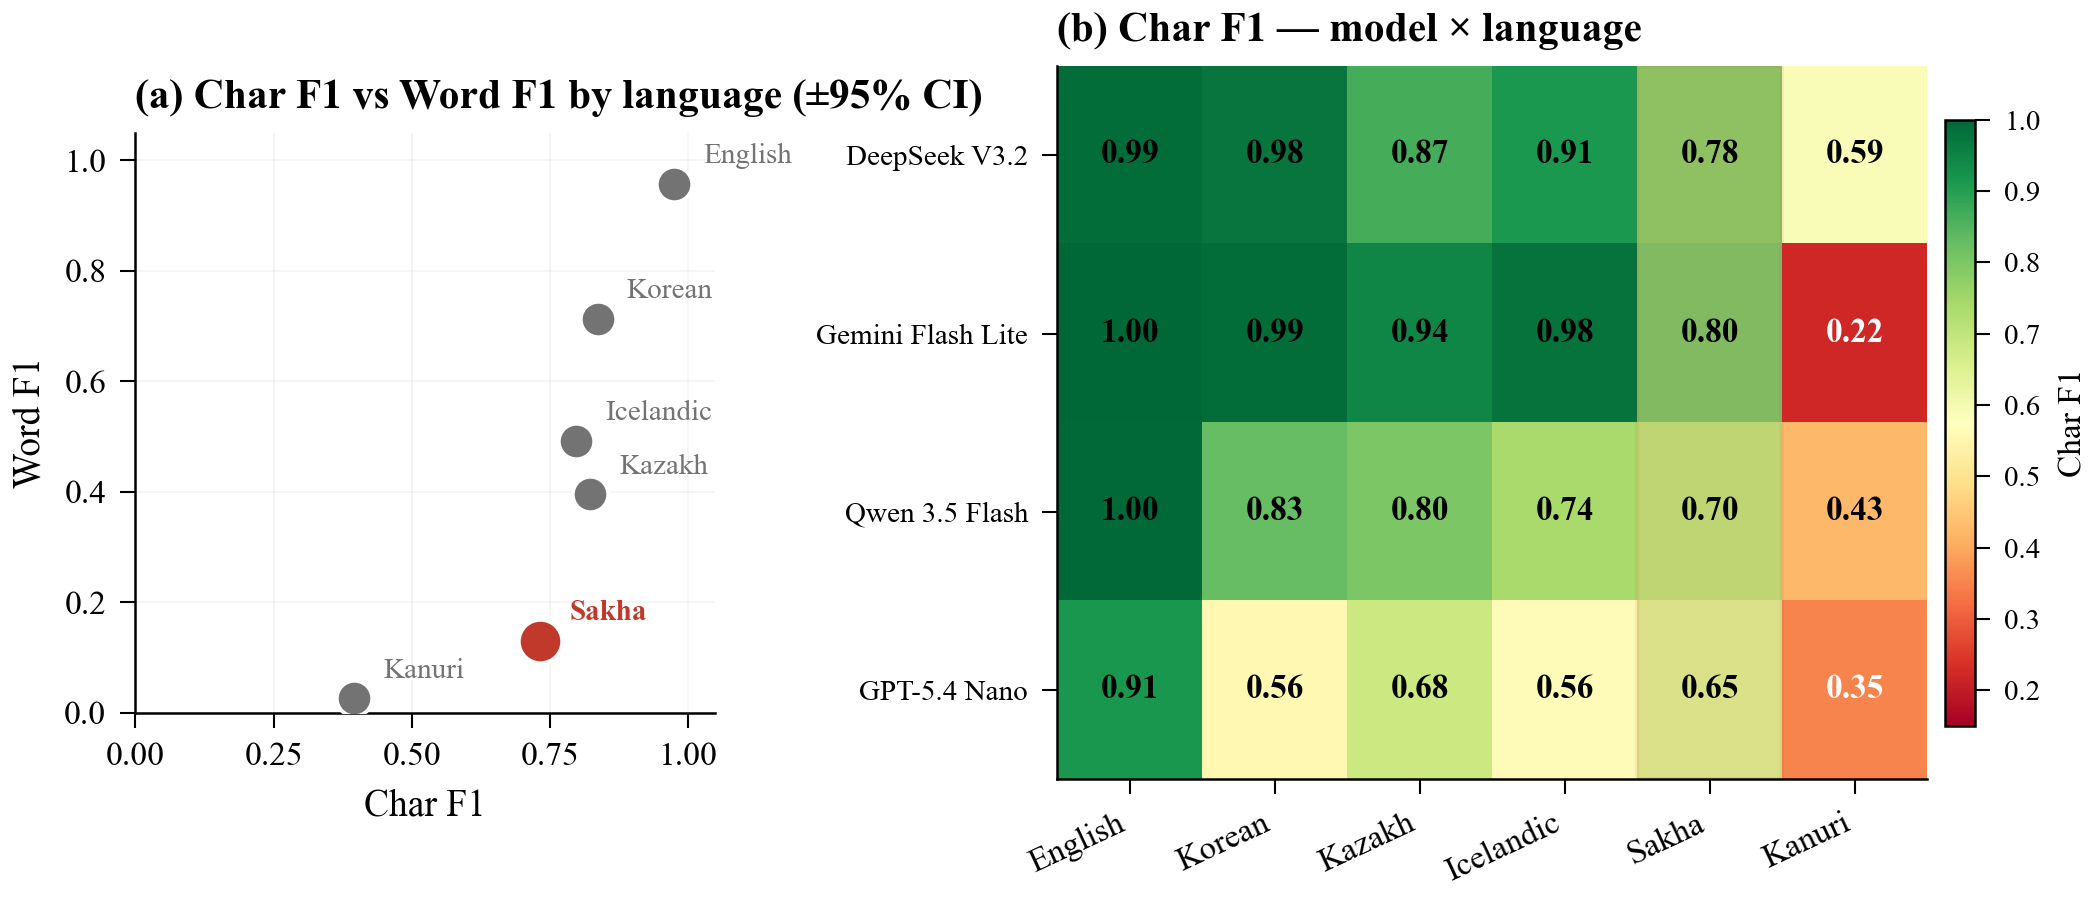
\includegraphics[width=1.0\textwidth]{plot3_sakha_cross_language.png}
    \caption{LLM performance on Sakha compared to other languages}
    \label{fig:plot3_sakha_cross_language}
\end{figure*}

\section{Discussion}

\subsection{Sakha in the resource continuum}

Performance on Sakha broadly tracks the resource classification scheme: the language sits 5th out of 6, comfortably above Class~0 Kanuri and clearly below Class~2 Icelandic and Class~3 Kazakh.
The wide gap to Kanuri ($+0.337$ Char F1, 95\% CI: $[+0.319,\ +0.356]$) confirms that even the modest digital footprint of a Class~1 language is sufficient for models to produce coherent output, whereas Class~0 represents a near-failure regime across all four models.

The gap to Kazakh ($-0.090$) is particularly notable.
Sakha and Kazakh share Turkic lineage and comparable typological features, yet Kazakh has orders-of-magnitude more web presence (Table~\ref{tab:language_resources}).
The performance gap is consistent with resource availability being a primary driver of model capability, independent of linguistic relatedness.

The Char~F1 / Word~F1 disparity distinctive to Sakha (and Kanuri) warrants closer attention.
Sakha's Word~F1 of 0.130 is an outlier relative to its Char~F1 of 0.733; by contrast, Kazakh and Icelandic show Char~F1 scores close to Sakha's but Word~F1 scores roughly three to four times higher.
Because the task measures reproduction of a canonical UDHR translation, high Word~F1 requires not merely correct language output but faithful replication of that specific document's wording.
For well-resourced languages the canonical text is likely present in training data, enabling near-verbatim recall; for Sakha, models produce continuations that diverge from the reference at the word level, yet may look plausible to a non-speaker.
The Char~F1 / Word~F1 gap therefore reflects the extent to which a model is generating rather than recalling, and Sakha's position in this gap is evidence of limited UDHR exposure rather than limited general language capability.

\subsection{Model and strategy differences}

Gemini~3.1 Flash Lite leads on every metric and also produces the lowest within-model variance (Char~F1 std\,=\,0.039), indicating consistently reliable output rather than occasional high-scoring generations.
Conversely, GPT-5.4~Nano's wide confidence intervals (std\,=\,0.184) reflect a bimodal pattern in which some samples are handled adequately while others fail almost entirely.
These differences are consistent across languages: Gemini is the most language-equitable model, with Sakha performance only 0.023 below its cross-language average.

One-shot prompting yields a statistically significant improvement over zero-shot, whereas the step from one-shot to few-shot is negligible in aggregate.
The effect is strongly model-dependent: GPT-5.4~Nano gains $+0.184$ Char~F1 with few-shot relative to zero-shot, while DeepSeek~V3.2 is essentially flat and Qwen~3.5~Flash shows a directionally negative trend under few-shot that approaches but does not cross the 95\% significance threshold.
Practitioners should therefore not assume a single best prompting strategy transfers across models for under-resourced languages.
Where a reference text is available, at least one-shot is advisable, but the model-specific interaction warrants empirical verification before deployment.

\subsection{Limitations}

Several design choices limit the generalisability of these findings.
The evaluation uses a single task (sentence continuation of one UDHR article) in a narrow legal-political register, which may not reflect model performance on conversational, literary, or technical Sakha text.
The design does not cover dedicated frontier and mid-tier models, limiting coverage of the full cost-quality curve.
All prompts were issued in English, leaving open the question of whether native-language prompting would alter results.
Automated string-similarity metrics, while deterministic and tokenizer-agnostic, are semantically blind: valid paraphrases are penalised equally with genuine errors.
Finally, the evaluation captures model behaviour at a single point in time; preview models such as Gemini~3.1 Flash-Lite may change before general availability, and all four models are subject to ongoing weight updates.

\subsection{Ethical considerations}

The evaluation corpus used in this study is freely available from the websites of the UN High Commissioner for Human Rights and the Ministry of Justice of the Republic of Kazakhstan. The corpus is in the public domain. No human subjects were involved.

Running inference across four LLMs incurs a noteable environmental footprint \cite{wu-etal-2025-unveiling}. We believe this cost is justified by establishing the first systematic cross-model benchmark for Sakha at minimal computational cost: the four models evaluated are all budget-tier (under \$0.30 per million input tokens) and the evaluation corpus is limited to a single UDHR article, making this one of the lowest-footprint benchmarking designs possible.

\subsection{Implications}

The results demonstrate that cost-efficient LLMs produce non-trivial Sakha output despite its Class~1 status, suggesting that resource class alone does not determine whether useful generation is achievable.
At the same time, the large gap to higher-resourced neighbours and the severe Word~F1 scores signal that current models fall well short of reliable Sakha fluency.
Closing that gap will likely require more Sakha text in training data rather than changes to model architecture or prompting alone.
For future evaluation work, the Char~F1 / Word~F1 disparity observed here motivates the use of generation-focused benchmarks (tasks where no canonical reference text exists) to more directly probe model capability in under-resourced languages.

\section{Conclusion}
Cost-efficient LLMs produce non-trivial Sakha output despite its Class 1 status, but fall well short of reliable fluency: the best model achieves a Char F1 of 0.799 and a Word F1 of only 0.27, versus 0.975 and 0.957 on English.
Performance tracks resource availability more strongly than linguistic relatedness, as Sakha lags Kazakh by 0.09 Char F1 despite shared Turkic ancestry.
The Char F1 / Word F1 disparity signals that models generate rather than recall Sakha text.
One-shot prompting helps on average, but its effect is model-dependent and can be neutral or slightly harmful, so practitioners should verify empirically rather than assume a single optimal strategy.
Improving Sakha performance will likely require more training data rather than architectural or prompting changes alone.

\bibliography{custom, anthology}

\end{document}
